%%%%%%%%%%%%%%%%%%%%%%%%%%%%%%%%%%%%
% 配布用ハンドアウト（解答なし）
% コンパイルコマンド: lualatex chp3_handout.tex
%%%%%%%%%%%%%%%%%%%%%%%%%%%%%%%%%%%%

\documentclass[slidestop,compress,mathserif,handout]{beamer}

% 解答を非表示にする
\newcommand{\soln}[1]{ }
\newcommand{\solnGr}[1]{ }

% 4スライドを1ページに印刷する設定
\usepackage{pgfpages}
\pgfpagesuselayout{4 on 1}[a4paper,landscape,border shrink=5mm]

%%%%%%%%%%%%%%%%%%%%%%%%%%%%%%%%%%%%
% 日本語サポート（LuaLaTeX使用）
%%%%%%%%%%%%%%%%%%%%%%%%%%%%%%%%%%%%

\usepackage{luatexja}
\usepackage{luatexja-fontspec}

%%%%%%%%%%%%%%%%%%%%%%%%%%%%%%%%%%%%
% スタイル
%%%%%%%%%%%%%%%%%%%%%%%%%%%%%%%%%%%%

\input{../lec_style_JP}

% 配布用：練習問題の正解を通常アイテムとして表示（オーバーレイなし）
\renewcommand{\solnMult}[1]{\item #1}

\setbeamertemplate{footline}{%
  \insertframenumber\,/\,\inserttotalframenumber}

%%%%%%%%%%%%%%%%%%%%%%%%%%%%%%%%%%%%
% プリアンブル
%%%%%%%%%%%%%%%%%%%%%%%%%%%%%%%%%%%%

\title[第3章：確率]{第3章：確率}
\author{OpenIntro Statistics 第4版（日本語版）}
\institute{$\:$ \\ {\footnotesize 原著スライド：Mine \c{C}etinkaya-Rundel（OpenIntro）\\
\webLink{http://creativecommons.org/licenses/by-sa/3.0/us/}{CC BY-SA ライセンス}のもと使用・翻訳。\\
一部の画像はフェアユース（教育目的）に基づき使用。}}
\date{}

%%%%%%%%%%%%%%%%%%%%%%%%%%%%%%%%%%%%
% ドキュメント開始
%%%%%%%%%%%%%%%%%%%%%%%%%%%%%%%%%%%%

\begin{document}


%%%%%%%%%%%%%%%%%%%%%%%%%%%%%%%%%%%%
% タイトルページ
%%%%%%%%%%%%%%%%%%%%%%%%%%%%%%%%%%%%

{
\addtocounter{framenumber}{-1}
{\removepagenumbers
\usebackgroundtemplate{
\includegraphics[width=\paperwidth]{../OpenIntro_Grid_4_3-01.jpg}}
\begin{frame}

\hfill 
\includegraphics[width=20mm]{../oiLogo_highres}

\titlepage

\end{frame}
}
}


%%%%%%%%%%%%%%%%%%%%%%%%%%%%%%%%%%%%
% 各節
%%%%%%%%%%%%%%%%%%%%%%%%%%%%%%%%%%%%

%%%%%%%%%%%%%%%%%%%%%%%%%%%%%%%%%%%%

\section{確率の定義}

%%%%%%%%%%%%%%%%%%%%%%%%%%%%%%%%%%%%

\subsection{確率}

%%%%%%%%%%%%%%%%%%%%%%%%%%%%%%%%%%%%

\begin{frame}
\frametitle{確率的プロセス}

\twocol{0.5}{0.5}
{
\begin{itemize}

\item \hl{確率的プロセス}とは、何が起こりうるかはわかっているが、実際にどの結果が起こるかわからない状況のことである。

\item 例：コイン投げ、サイコロの目、iTunes シャッフル、明日の株式市場の上下など。

\item 実際には確率的でなくても、プロセスを確率的にモデル化することが有用な場合がある。

\end{itemize}
}{
\begin{center}
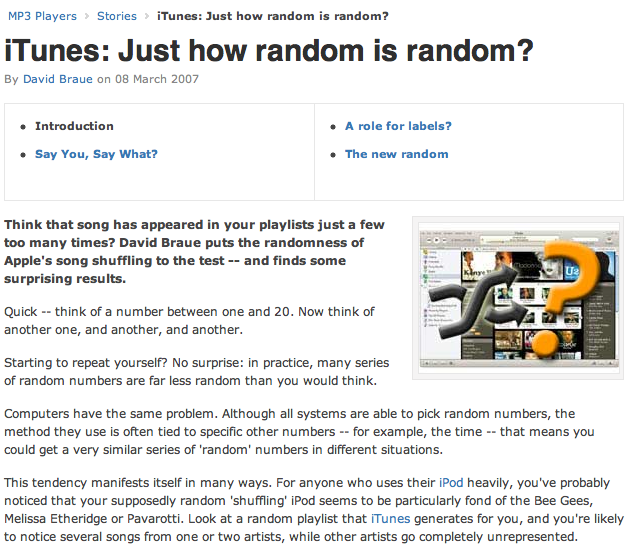
\includegraphics[width=\textwidth]{3-1_define_probability/figures/iTunes}
\end{center}
\ct{ \webURL{http://www.cnet.com.au/itunes-just-how-random-is-random-339274094.htm}}
}

\end{frame}

%%%%%%%%%%%%%%%%%%%%%%%%%%%%%%%%%%%%

\begin{frame}
\frametitle{確率}

\begin{itemize}

\item 確率にはいくつかの解釈があるが、確率が従うべき数学的規則についてはほぼ完全に一致している。
\begin{itemize}
\item $P(A)$ = 事象 A の確率
\item $0 \le P(A) \le 1$
\end{itemize}

\item \hl{頻度論的解釈：}
\begin{itemize}
\item ある結果の確率は、確率的プロセスを無限回観察したときにその結果が起こる割合である。
\end{itemize}

\item \hl{ベイズ的解釈：}
\begin{itemize}
\item ベイズ主義者は確率を主観的な信念の度合いとして解釈する：同じ事象でも、異なる人が異なる確率を割り当てることがある。
\item 過去20年間の計算技術と方法の革命的進歩によって広まった。
\end{itemize}

\end{itemize}

\end{frame}

%%%%%%%%%%%%%%%%%%%%%%%%%%%%%%%%%%%%

\begin{frame}[shrink=25]
\frametitle{練習問題}

\pq{次のどの事象が最も驚くべきものか？}

\begin{enumerate}[(a)]
\item 10回コインを投げて、ちょうど3回表が出る
\item 100回コインを投げて、ちょうど3回表が出る
\solnMult{1000回コインを投げて、ちょうど3回表が出る}
\end{enumerate}

\end{frame}

%%%%%%%%%%%%%%%%%%%%%%%%%%%%%%%%%%%%

\begin{frame}
\frametitle{大数の法則}

\hl{大数の法則}とは、観測数が増えるにつれて、ある特定の結果が起こる割合 \mathhl{\hat{p}_n} が、その結果の確率 \mathhl{p} に収束することを述べたものである。

\end{frame}

%%%%%%%%%%%%%%%%%%%%%%%%%%%%%%%%%%%%

\begin{frame}[shrink=15]
\frametitle{大数の法則（続き）}

\dq{\textit{公正な}コインを投げたとき、最初の10回すべてで表が出た場合、次の投げで表が出る確率はいくつだと思うか？ 0.5、0.5より小さい、それとも0.5より大きい？}

\[ \underline{H} \hspace{1mm} \underline{H} \hspace{1mm} \underline{H} \hspace{1mm} \underline{H} \hspace{1mm} \underline{H} \hspace{1mm} \underline{H} \hspace{1mm} \underline{H} \hspace{1mm} \underline{H} \hspace{1mm} \underline{H} \hspace{1mm} \underline{H} \hspace{1mm} \underline{?} \]

\begin{itemize}
\item 確率はやはり 0.5 であり、次の投げで表が出る確率は 50\% である。
\[ P(H \text{ on 11}^{th} \text{ toss}) = P(T \text{ on 11}^{th} \text{ toss}) = 0.5 \]
\item コインは「裏を出すべき」ではない。
\item 大数の法則についての一般的な誤解は、確率的プロセスは過去に起こったことを補正するはずだというものであるが、これは誤りであり、\hl{ギャンブラーの誤謬}（または\hl{平均の法則}）とも呼ばれる。
\end{itemize}

\end{frame}

%%%%%%%%%%%%%%%%%%%%%%%%%%%%%%%%%%%%

\subsection{互いに排反な結果}

%%%%%%%%%%%%%%%%%%%%%%%%%%%%%%%%%%%%

\begin{frame}[shrink=10]
\frametitle{互いに排反な結果とそうでない結果}

\hl{互いに排反（mutually exclusive）な結果：}同時には起こり得ない。
\begin{itemize}
\item 1回のコイン投げの結果が表と裏の両方になることはない。
\item 学生が同じ科目で合格と不合格の両方になることはない。
\item 1枚のカードがエースとクイーンの両方であることはない。
\end{itemize}

\hl{互いに排反でない結果：}同時に起こり得る。
\begin{itemize}
\item 学生が同じ学期に統計学でA、経済学でAをとることがある。
\end{itemize}

\end{frame}

%%%%%%%%%%%%%%%%%%%%%%%%%%%%%%%%%%%%

\begin{frame}[shrink=10]
\frametitle{互いに排反でない事象の和事象}

\dq{よくシャッフルされた1組のトランプから、ジャックまたは赤いカードを引く確率は何か？}

\begin{figure}
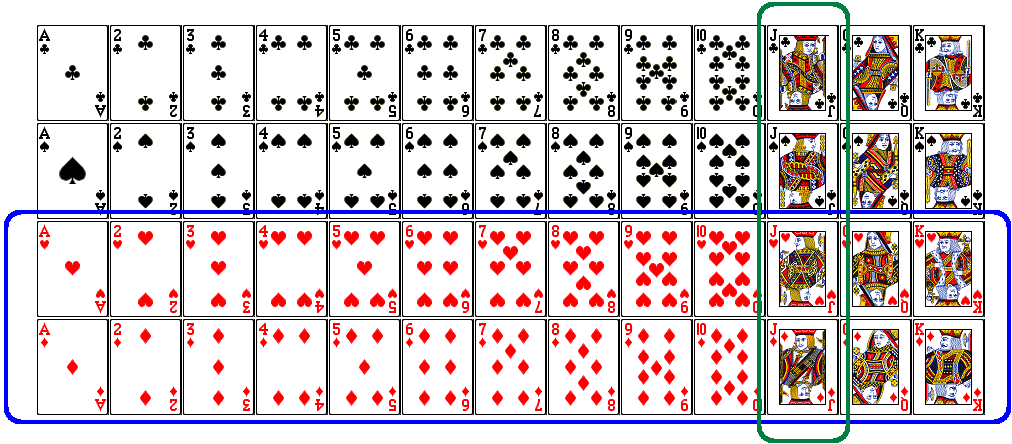
\includegraphics[width=0.7\textwidth]{3-1_define_probability/figures/cards}
\end{figure}

\vspace{-0.75cm}

\soln{
\begin{align*}
P(\text{ジャックまたは赤}) &= P(\text{ジャック}) + P(\text{赤}) - \orange{$P(\text{ジャックかつ赤})$} \\
&= \frac{4}{52} + \frac{26}{52} - \frac{2}{52} = \frac{28}{52}
\end{align*}
}

\vfill

\ct{Figure from \webURL{http://www.milefoot.com/math/discrete/counting/cardfreq.htm}.}

\end{frame}

%%%%%%%%%%%%%%%%%%%%%%%%%%%%%%%%%%%%

\subsection{事象が互いに排反でない場合の確率}

%%%%%%%%%%%%%%%%%%%%%%%%%%%%%%%%%%%%

\begin{frame}
\frametitle{練習問題}

\pq{無作為に選ばれた学生が、大麻を合法化すべきと考えている\underline{か}、または親の政治的見解に同意している確率は何か？}

{\small
\begin{center}
\begin{tabular}{l  cc c}
            & \multicolumn{2}{c}{\textit{親の政治観に同意}} & \\
\cline{2-3}
\textit{大麻合法化} & なし & あり & 合計 \\
\hline
反対          & 11 & 40 & 51 \\
賛成         & 36 & 78 & 114 \\
\hline
合計       & 47 & 118 & 165
\end{tabular}
\end{center}
}

\begin{enumerate}[(a)]
\item $\frac{40 + 36 - 78}{165}$
\solnMult{$\frac{114 + 118 - 78}{165}$}
\item $\frac{78}{165}$
\item $\frac{78}{188}$
\item $\frac{11}{47}$
\end{enumerate}

\end{frame}

%%%%%%%%%%%%%%%%%%%%%%%%%%%%%%%%%%%%

\begin{frame}
\frametitle{まとめ}

\formula{一般加法定則}{\[ P(A~\text{または}~B) = P(A) + P(B) - P(A~\text{かつ}~B) \]}

\Note{互いに排反な事象では $P(A~\text{かつ}~B) = 0$ なので、上式は $P(A~\text{または}~B) = P(A) + P(B)$ に簡略化される。}

\end{frame}

%%%%%%%%%%%%%%%%%%%%%%%%%%%%%%%%%%%%

\subsection{確率分布}

%%%%%%%%%%%%%%%%%%%%%%%%%%%%%%%%%%%%

\begin{frame}
\frametitle{確率分布}

\hl{確率分布}は、起こりうるすべての事象とそれらが起こる確率を一覧にしたものである。

\begin{itemize}
\item 1人の子どもの性別の確率分布：
{\footnotesize
\begin{center}
\begin{tabular}{r | c | c}
事象    & 男		& 女 \\
\hline
確率	& 0.5		& 0.5 \\
\end{tabular}
\end{center}
}

\item 確率分布の規則：
\begin{enumerate}
\item 列挙された事象は互いに排反でなければならない
\item 各確率は0以上1以下でなければならない
\item 確率の合計は1でなければならない
\end{enumerate}

\item 2人の子どもの性別の確率分布：
\soln{
{\footnotesize
\begin{center}
\begin{tabular}{r | c | c | c | c}
事象		& MM	& FF		& MF		& FM \\
\hline
確率	& 0.25	& 0.25	& 0.25	& 0.25 \\
\end{tabular}
\end{center}
}}

\end{itemize}

\end{frame}

%%%%%%%%%%%%%%%%%%%%%%%%%%%%%%%%%%%%

\begin{frame}
\frametitle{練習問題}

\pq{調査で、回答者の52\%が民主党員だと答えた。このサンプルから無作為に選ばれた回答者が共和党員である確率はいくつか？}

\begin{enumerate}[(a)]
\item 0.48
\item 0.48より大きい
\item 0.48より小さい
\solnMult{与えられた情報だけでは計算できない}
\end{enumerate}

\only<2->{\orange{唯一の2つの政党が共和党と民主党である場合は (a) が可能である。しかし、政党に所属しない人やこれら2つ以外の政党に所属する人もいる可能性があるため、(c) も可能である。(b) は合計確率が1を超えることになるため、絶対に不可能である。}}

\end{frame}

%%%%%%%%%%%%%%%%%%%%%%%%%%%%%%%%%%%%

\subsection{余事象}

%%%%%%%%%%%%%%%%%%%%%%%%%%%%%%%%%%%%

\begin{frame}
\frametitle{標本空間と余事象}

\hl{標本空間}は、試行で起こりうるすべての結果の集合である。

\begin{itemize}
\item ある夫婦に1人の子どもがいる場合、その性別の標本空間は？ $S = \{ M, F \}$
\item ある夫婦に2人の子どもがいる場合、その性別の標本空間は？ \soln{$S = \{ MM, FF, FM, MF \}$}
\end{itemize}

\hl{余事象}は、確率の和が1になる2つの互いに排反な事象である。

\begin{itemize}
\item ある夫婦に1人の子どもがいる。その子が男の子でないとわかった場合、その性別は？
\{ \sout{\textcolor{gray}{M}}, \orange{F} \} $\rightarrow$ 男の子と女の子は\hl{余事象}である。
\item ある夫婦に2人の子どもがいる。両方が女の子でないとわかった場合、可能な性別の組み合わせは？
\soln{\{ \orange{MM}, \sout{\textcolor{gray}{FF}}, \orange{FM}, \orange{MF} \} }
\end{itemize}

\end{frame}

%%%%%%%%%%%%%%%%%%%%%%%%%%%%%%%%%%%%

\subsection{独立}

%%%%%%%%%%%%%%%%%%%%%%%%%%%%%%%%%%%%

\begin{frame}
\frametitle{独立}

2つのプロセスが\hl{独立}であるとは、一方の結果を知っても他方の結果についての有用な情報が得られない場合をいう。

\begin{itemize}

\item 最初の投げでコインが表になったことを知っても、2回目の投げでコインがどちらになるかについての有用な情報は得られない。$\rightarrow$ 2回のコイン投げの結果は独立である。

\item 最初に引いたカードがエースであることを知ると、2回目の引きでエースを引く確率についての有用な情報が得られる。$\rightarrow$ デッキからの2回の引き（非復元）の結果は従属である。

\end{itemize}

\end{frame}

%%%%%%%%%%%%%%%%%%%%%%%%%%%%%%%%%%%%

\begin{frame}
\frametitle{練習問題}

\pq{\small{2013年1月9日〜12日、SurveyUSA がノースカロライナ州の居住者500人の無作為標本を対象に、銃の広範な所有は法を守る市民を犯罪から守るか、社会をより危険にするかを質問した。回答者全体の58\%が「市民を守る」と回答した。白人回答者の67\%、黒人回答者の28\%、ヒスパニック回答者の64\%がこの見解を共有していた。次のうち正しいものはどれか？}}

銃所有に関する意見と人種・民族は最も可能性が高いのは
\begin{enumerate}[(a)]
\item 余事象
\item 互いに排反
\item 独立
\solnMult{従属}
\item 互いに排反
\end{enumerate}

\ct{\webURL{http://www.surveyusa.com/client/PollReport.aspx?g=a5f460ef-bba9-484b-8579-1101ea26421b}}

\end{frame}

%%%%%%%%%%%%%%%%%%%%%%%%%%%%%%%%%%%%

\begin{frame}[shrink=15]
\frametitle{}

\formula{独立性の確認}{P(B が真であるとき A が起こる) = $P(A~|~B) = P(A)$ ならば、A と B は独立である。}

$\:$ \\

\soln{P(市民を守る) = 0.58 \\
$\:$ \\
P(無作為に選ばれたノースカロライナ州居住者が銃所有は市民を守ると答える，その居住者が白人である場合) = \\ P(市民を守る $|$ 白人) = 0.67 \\
$\:$ \\
P(市民を守る $|$ 黒人) = 0.28 \\
$\:$ \\
P(市民を守る $|$ ヒスパニック) = 0.64 \\
$\:$ \\
P(市民を守る) は人種・民族によって異なるため、銃所有に関する意見と人種・民族は最も可能性が高いのは従属である。
}

\end{frame}

%%%%%%%%%%%%%%%%%%%%%%%%%%%%%%%%%%%%

\begin{frame}[shrink=10]
\frametitle{標本データに基づく従属性の判定}

\begin{itemize}

\item 標本データから計算された条件付き確率が2つの変数間の従属性を示している場合、次のステップは、確率の観測された差が偶然に起こる可能性があるかを判定する仮説検定を行うことである。

\item 条件付き確率間の観測された差が大きいほど、その差が真であるという証拠が強くなる。

\item 標本が大きい場合、小さな差でも真の差の強い証拠となりうる。

\end{itemize}

\dq{{\small P(市民を守る $|$ 白人) = 0.67、P(市民を守る $|$ ヒスパニック) = 0.64 であった。白人とヒスパニックで銃の広範な所有が市民を守ると思う割合に真の差があると確信するのはどちらの条件下か？ $n = 500$ か $n = 50,000$ か？}} \soln{$n = 50,000$}

\end{frame}

%%%%%%%%%%%%%%%%%%%%%%%%%%%%%%%%%%%%

\begin{frame}
\frametitle{}

\formula{独立事象の積の法則}{\[P(A~\text{かつ}~B) = P(A) \times P(B) \]
\small{より一般的には、$P(A_1~\text{かつ}~\cdots~\text{かつ}~A_k) = P(A_1) \times \cdots \times P(A_k)$}}

\dq{コインを2回投げるとき、2回続けて裏が出る確率は何か？}

\[ P(\text{1回目に裏}) \times  P(\text{2回目に裏}) = \frac{1}{2} \times \frac{1}{2} = \frac{1}{4} \]

\end{frame}

%%%%%%%%%%%%%%%%%%%%%%%%%%%%%%%%%%%%

\begin{frame}[shrink=10]
\frametitle{練習問題}

\pq{最近のギャラップ調査によると、2012年6月時点でテキサス州民の25.5\%が健康保険を持っていない。非加入率が一定であると仮定して、無作為に選んだ2人のテキサス州民が両方とも非加入である確率は何か？}

\twocol{0.4}{0.6}
{
\begin{enumerate}[(a)]
\item $25.5^2$
\solnMult{$0.255^2$}
\item $0.255 \times 2$
\item $(1 - 0.255)^2$
\end{enumerate}
}
{
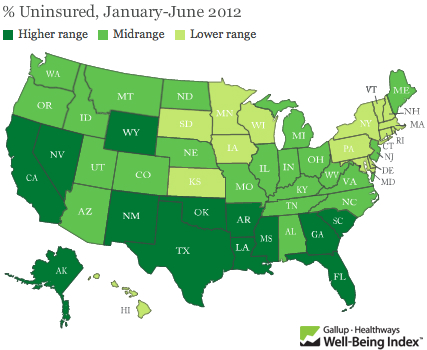
\includegraphics[width=0.9\textwidth]{3-1_define_probability/figures/uninsured}
}

\ct{ \webURL{http://www.gallup.com/poll/156851/uninsured-rate-stable-across-states-far-2012.aspx}}

\end{frame}

%%%%%%%%%%%%%%%%%%%%%%%%%%%%%%%%%%%%

\subsection{まとめ}

%%%%%%%%%%%%%%%%%%%%%%%%%%%%%%%%%%%%

\begin{frame}
\frametitle{互いに排反 vs. 余事象}

\dq{2つの互いに排反な事象の確率の和は常に1になるか？}

\soln{必ずしもそうではない。標本空間に3つ以上の事象がある場合がある（例：党派）。}

$\:$ \\

\dq{2つの余事象の確率の和は常に1になるか？}

\soln{はい、それが余事象の定義である（例：表と裏）。}

\end{frame}

%%%%%%%%%%%%%%%%%%%%%%%%%%%%%%%%%%%%

\begin{frame}
\frametitle{すべてをまとめると…}

\dq{テキサス州民を5人無作為に選ぶとき、少なくとも1人が保険未加入である確率は何か？}

\begin{itemize}

\item テキサス州民を5人無作為に選んだ場合、保険未加入者の人数の標本空間は：
\[ S = \{0, 1, 2, 3, 4, 5\} \]

\item 少なくとも1人が保険未加入である場合に注目する：
\[ S = \{0, \orange{$1, 2, 3, 4, 5$} \} \]

\item 標本空間を2つのカテゴリに分割できる：
\[ S = \{0, \orange{\text{少なくとも1人}} \} \]

\end{itemize}

\end{frame}

%%%%%%%%%%%%%%%%%%%%%%%%%%%%%%%%%%%%

\begin{frame}[shrink=10]
\frametitle{すべてをまとめると…}

標本空間の確率の和は1でなければならないため：
\begin{eqnarray*}
P(\text{少なくとも1人が未加入}) &=& 1 - P(\text{未加入者なし}) \\
&=& 1 - [(1-0.255)^5] \\
&=& 1- 0.745^5 \\
&=& 1 - 0.23 \\
&=& 0.77
\end{eqnarray*}

$\:$ \\
$\:$ \\

\formula{少なくとも1}{\[P(\text{少なくとも1}) = 1 - P(\text{1つもない})\]}

\end{frame}

%%%%%%%%%%%%%%%%%%%%%%%%%%%%%%%%%%%%

\begin{frame}
\frametitle{練習問題}

\pq{ある大学の学部生の約20\%がベジタリアンまたはビーガンである。学部生3人の無作為標本から、少なくとも1人がベジタリアンまたはビーガンである確率は何か？}

\twocol{0.3}{0.6}{
\begin{enumerate}[(a)]
\item $1 - 0.2 \times 3$
\item $1 - 0.2^3$
\item $0.8^3$
\item $1 - 0.8 \times 3$
\solnMult{$1 - 0.8^3$}
\end{enumerate}
}
{
\soln{
$P(\text{少なくとも1人がベジタリアン}) = 1- P(\text{ベジタリアンなし})$ \\
$= 1 - (1 - 0.2)^3$ \\
$= 1 - 0.8^3$ \\
$= 1 - 0.512 = 0.488$ }
}

\end{frame}

%%%%%%%%%%%%%%%%%%%%%%%%%%%%%%%%%%%%

%%%%%%%%%%%%%%%%%%%%%%%%%%%%%%%%%%%%

\section{条件付き確率}

%%%%%%%%%%%%%%%%%%%%%%%%%%%%%%%%%%%%

\subsection{分割表を用いた確率の探索}

%%%%%%%%%%%%%%%%%%%%%%%%%%%%%%%%%%%%

\begin{frame}
\frametitle{再発}

研究者たちは、コカイン慢性使用者72人を3つのグループに無作為に割り当てた：デシプラミン（抗うつ薬）、リチウム（コカインの標準治療）、プラセボ。研究結果を以下にまとめる。

{\small
\begin{center}
\begin{tabular}{l | c c | c}
			& 		& 再発 		&  \\
			& 再発あり	& なし	& 合計 \\
\hline
デシプラミン	& 10		& 14		& 24 \\
リチウム		& 18		& 6		& 24 \\
プラセボ		& 20		& 4		& 24 \\
\hline
合計			& 48		& 24		& 72
\end{tabular}
\end{center}
}

\ct{\webURL{http://www.oswego.edu/~srp/stats/2_way_tbl_1.htm}}

\end{frame}

%%%%%%%%%%%%%%%%%%%%%%%%%%%%%%%%%%%%

\begin{frame}

\dq{患者が再発しなかった確率は何か？}


{\small
\begin{center}
\begin{tabular}{l | c c | c}
			& 		& 再発 		&  \\
			& 再発あり	& なし	& 合計 \\
\hline
デシプラミン	& 10		& 14		& 24 \\
リチウム		& 18		& 6		& 24 \\
プラセボ		& 20		& 4		& 24 \\
\hline
合計			& 48		& 24		& 72
\end{tabular}
\end{center}
}

\end{frame}

%%%%%%%%%%%%%%%%%%%%%%%%%%%%%%%%%%%%

\subsection{周辺確率と結合確率}

%%%%%%%%%%%%%%%%%%%%%%%%%%%%%%%%%%%%

\begin{frame}
\frametitle{周辺確率}

\dq{患者が再発した確率は何か？}

{\small
\begin{center}
\begin{tabular}{l | c c | c}
			& 		& 再発 		&  \\
			& 再発あり	& なし	& 合計 \\
\hline
デシプラミン	& 10		& 14		& 24 \\
リチウム		& 18		& 6		& 24 \\
プラセボ		& 20		& 4		& 24 \\
\hline
合計			& \red{48}		& 24		& \red{72}
\end{tabular}
\end{center}
}

P(再発あり) = $\frac{48}{72} \approx 0.67$ \\

\end{frame}

%%%%%%%%%%%%%%%%%%%%%%%%%%%%%%%%%%%%

\begin{frame}
\frametitle{結合確率}

\dq{患者が抗うつ薬（デシプラミン）を投与された\underline{かつ}再発した確率は何か？}

{\small
\begin{center}
\begin{tabular}{l | c c | c}
			& 		& 再発 		&  \\
			& 再発あり	& なし	& 合計 \\
\hline
デシプラミン	& \red{10}		& 14		& 24 \\
リチウム		& 18		& 6		& 24 \\
プラセボ		& 20		& 4		& 24 \\
\hline
合計			& 48	& 24		& \red{72}
\end{tabular}
\end{center}
}

P(再発あり かつ デシプラミン) = $\frac{10}{72} \approx 0.14$ \\

\end{frame}

%%%%%%%%%%%%%%%%%%%%%%%%%%%%%%%%%%%%

\subsection{条件付き確率の定義}

%%%%%%%%%%%%%%%%%%%%%%%%%%%%%%%%%%%%

\begin{frame}[shrink=10]
\frametitle{条件付き確率}

\formula{条件付き確率}{
条件 $B$ のもとで目的の結果 $A$ が起こる条件付き確率は次のように計算される
\[ P(A|B) = \frac{P(A~\text{かつ}~B)}{P(B)} \]
}

\twocol{0.5}{0.5}
{
{\small
\begin{center}
\begin{tabular}{l | c c | c}
			& 		& 再発 		&  \\
			& 再発あり	& なし	& 合計 \\
\hline
デシプラミン	& 10		& 14		& 24 \\
リチウム		& 18		& 6		& 24 \\
プラセボ		& 20		& 4		& 24  \\
\hline
合計			& 48		& 24		&  72
\end{tabular}
\end{center}
}
}
{
\begin{eqnarray*}
&&P(\text{再発} |  \text{デシプラミン}) \\
&&= \frac{P(\text{再発} ~ \text{かつ} ~ \text{デシプラミン})}{P(\text{デシプラミン})} \\
&&= \frac{10 / 72}{24 / 72} \\
&&= \frac{10}{24} \\
&&= 0.42
\end{eqnarray*}
}

\end{frame}

%%%%%%%%%%%%%%%%%%%%%%%%%%%%%%%%%%%%

\begin{frame}
\frametitle{条件付き確率（続き）}

\dq{患者が抗うつ薬（デシプラミン）を投与されたとわかっている場合、再発した確率は何か？}

{\small
\begin{center}
\begin{tabular}{l | c c | c}
			& 		& 再発 		&  \\
			& 再発あり	& なし	& 合計 \\
\hline
\rowcolor[gray]{.7}
デシプラミン	& \red{10}			& 14		& \red{24} \\
リチウム		& 18		& 6		& 24 \\
プラセボ		& 20 		& 4		& 24  \\
\hline
合計			& 48	& 24		&  72
\end{tabular}
\end{center}
}

P(再発 $|$ デシプラミン) = $\frac{10}{24} \approx 0.42$ \\

$\:$ \\
P(再発 $|$ リチウム) = $\frac{18}{24} \approx 0.75$ \\
P(再発 $|$ プラセボ) = $\frac{20}{24} \approx 0.83$ \\

\end{frame}

%%%%%%%%%%%%%%%%%%%%%%%%%%%%%%%%%%%%

\begin{frame}
\frametitle{条件付き確率（続き）}

\dq{患者が再発したとわかっている場合、抗うつ薬（デシプラミン）を投与されていた確率は何か？}

{\small
\begin{center}
\begin{tabular}{l | >{\columncolor[gray]{0.7}[0pt]}c c | c}
			& 		& 再発 		&  \\
			& 再発あり	& なし	& 合計 \\
\hline
デシプラミン	& \red{10}			& 14		& 24 \\
リチウム		& 18		& 6		& 24 \\
プラセボ		& 20		& 4		& 24  \\
\hline
合計			& \red{48}	& 24		&  72
\end{tabular}
\end{center}
}

P(デシプラミン $|$ 再発) = $\frac{10}{48} \approx 0.21$ \\

$\:$ \\
P(リチウム $|$ 再発) = $\frac{18}{48} \approx 0.375$ \\
P(プラセボ $|$ 再発) = $\frac{20}{48} \approx 0.42$ \\

\end{frame}

%%%%%%%%%%%%%%%%%%%%%%%%%%%%%%%%%%%%

\subsection{一般乗法定則}

%%%%%%%%%%%%%%%%%%%%%%%%%%%%%%%%%%%%

\begin{frame}
\frametitle{一般乗法定則}

\begin{itemize}

\item 2つの事象が独立である場合、その結合確率は単純にそれぞれの確率の積であることを見た。事象が独立でないと考えられる場合、結合確率は少し異なる方法で計算される。

\item $A$ と $B$ が2つの結果または事象を表す場合、
\formula{\[ P(A~\text{かつ}~B) = P(A|B) \times P(B) \]}
この式は、条件付き確率の公式を変形したものに過ぎない。

\item $A$ を目的の結果、$B$ を条件として考えると便利である。

\end{itemize}

\end{frame}

%%%%%%%%%%%%%%%%%%%%%%%%%%%%%%%%%%%%

\subsection{条件付き確率における独立性の考慮}

%%%%%%%%%%%%%%%%%%%%%%%%%%%%%%%%%%%%

\begin{frame}[shrink=10]
\frametitle{独立性と条件付き確率}

以下は、入門統計学クラスの学生の性別と専攻の（仮想の）分布である：

{\small
\begin{center}
\begin{tabular}{l | c c | c}
			& 社会	& 非社会 		&  \\
			& 科学	& 科学	& 合計 \\
\hline
女性		& 30		& 20		& 50 \\
男性			& 30		& 20		& 50 \\
\hline
合計			& 60		& 40		& 100
\end{tabular}
\end{center}
}

\begin{itemize}

\item 無作為に選ばれた学生が社会科学専攻である確率は $\frac{60}{100} = 0.6$。

\item 無作為に選ばれた学生が女性であるとわかっている場合、社会科学専攻である確率は $\frac{30}{50} = 0.6$。

\item $P(SS | M)$ も 0.6 に等しいため、このクラスの学生の専攻は性別に依存しない：P(SS $|$ F) = P(SS)。

\end{itemize}

\end{frame}

%%%%%%%%%%%%%%%%%%%%%%%%%%%%%%%%%%%%

\begin{frame}
\frametitle{独立性と条件付き確率（続き）}

一般的に、$P(A|B) = P(A)$ であれば、事象 $A$ と $B$ は独立であるといわれる。

\begin{itemize}

\item 概念的に：$B$ を与えても $A$ について何も教えてくれない。

\item 数学的に：事象 $A$ と $B$ が独立であれば $P(A~\text{かつ}~B) = P(A) \times P(B)$ であることがわかっている。すると、
\[ P(A|B) = \frac{P(A~\text{かつ}~B)}{P(B)} = \frac{P(A) \times P(B)}{P(B)} = P(A) \]

\end{itemize}

\end{frame}

%%%%%%%%%%%%%%%%%%%%%%%%%%%%%%%%%%%%

\subsection{樹形図}

%%%%%%%%%%%%%%%%%%%%%%%%%%%%%%%%%%%%

\begin{frame}[shrink=25]
\frametitle{乳がん検診}

\begin{itemize}

\item 米国がん協会の推定によれば、女性の約1.7\%が乳がんを患っている。 \\
{\small\webURL{http://www.cancer.org/cancer/cancerbasics/cancer-prevalence}}

\item Susan G. Komen For The Cure Foundation によれば、マンモグラフィは実際に乳がんを患っている女性の約78\%を正確に識別する。 \\
{\small\webURL{http://ww5.komen.org/BreastCancer/AccuracyofMammograms.html}}

\item 2003年に発表された論文によれば、すべてのマンモグラフィのうち最大10\%ががんを患っていない患者に対して偽陽性を示す。 \\{\small \webURL{http://www.ncbi.nlm.nih.gov/pmc/articles/PMC1360940}}

\end{itemize}

\vfill

\Note{これらの割合は近似値であり、推定が非常に難しい。}

\end{frame}

%%%%%%%%%%%%%%%%%%%%%%%%%%%%%%%%%%%

\begin{frame}[shrink=10]
\frametitle{確率の逆転}

\dq{患者が乳がん検診を受けるとき、2つの競合する主張がある：患者はがんである、患者はがんでない。マンモグラフィが陽性の結果を示した場合、患者が実際にがんである確率は何か？}

\twocol{0.7}{0.3}{
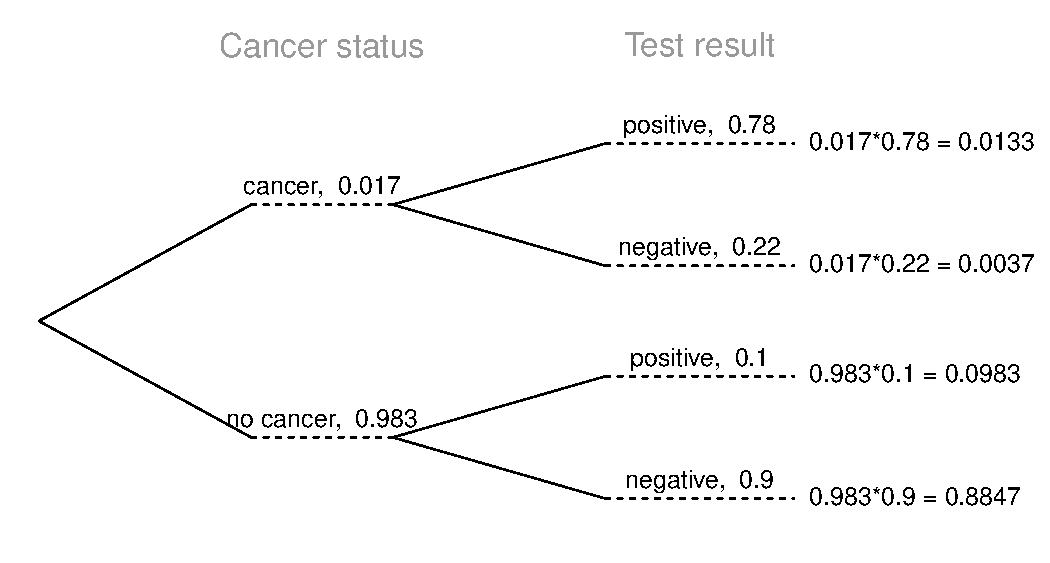
\includegraphics[width=\textwidth]{3-2_conditional_probability/figures/cancer_tree/cancer_tree_first}
}
{
{\footnotesize
\begin{eqnarray*}
&&P(C | +) \\
&&= \frac{P(C~\text{かつ}~+)}{P(+)} \\
&&= \frac{0.0133}{0.0133 + 0.0983} \\
&&= 0.12
\end{eqnarray*}
}
}

\Note{樹形図は確率を逆転させるのに有用である：$P(+|C)$ が与えられ、$P(C|+)$ を求める。}

\end{frame}

%%%%%%%%%%%%%%%%%%%%%%%%%%%%%%%%%%%

\begin{frame}
\frametitle{練習問題}

\pq{1回検査を受けて陽性の結果を得た女性が再検査を受けたいとする。2回目の検査では、この特定の女性ががんである確率はいくつと仮定すべきか？}

\begin{enumerate}[(a)]
\item 0.017
\solnMult{0.12}
\item 0.0133
\item 0.88
\end{enumerate}

\end{frame}

%%%%%%%%%%%%%%%%%%%%%%%%%%%%%%%%%%%

\begin{frame}
\frametitle{練習問題}

\pq{この2回目のマンモグラフィでも陽性の結果が出た場合、この女性ががんである確率は何か？}

\twocol{0.2}{0.7}
{
\begin{enumerate}[(a)]
\item 0.0936
\item 0.088
\item 0.48
\solnMult{0.52}
\end{enumerate}
}
{
\solnGr{
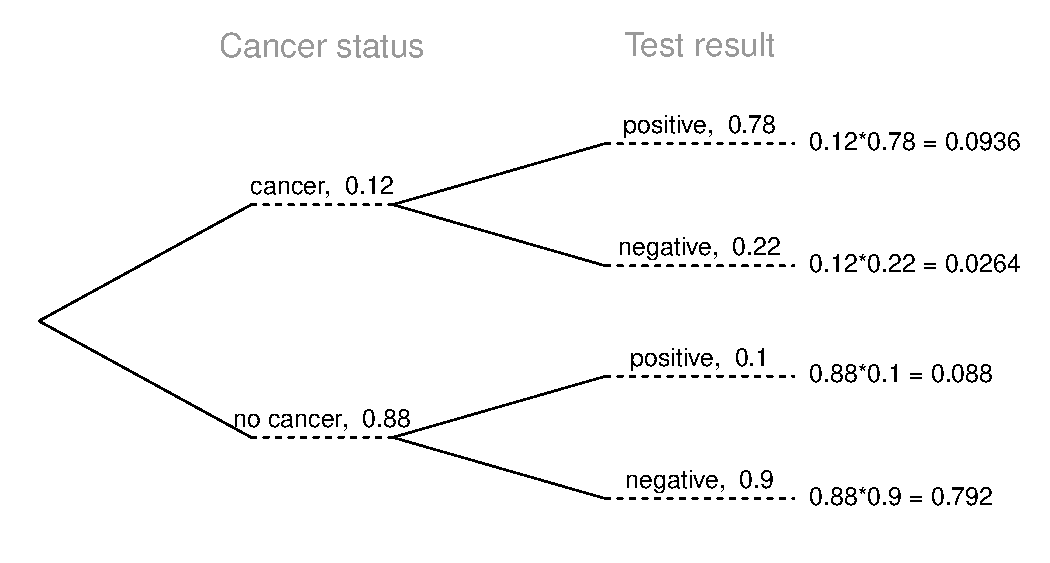
\includegraphics[width=\textwidth]{3-2_conditional_probability/figures/cancer_tree/cancer_tree_second}
}
}

\soln{
{\small \[P(C | +) = \frac{P(C~\text{かつ}~+)}{P(+)} = \frac{0.0936}{0.0936+0.088} = 0.52\]}
}

\end{frame}

%%%%%%%%%%%%%%%%%%%%%%%%%%%%%%%%%%%

\subsection{ベイズの定理}

%%%%%%%%%%%%%%%%%%%%%%%%%%%%%%%%%%%%

\begin{frame}
\frametitle{ベイズの定理}

\begin{itemize}

\item これまで見てきた条件付き確率の公式は、ベイズの定理の特殊な場合であり、事象が2つ以上の結果を持つ場合にも適用できる。

\item \hl{ベイズの定理：}
\formula{
\[ P(\text{変数1の結果}~A_1~|~\text{変数2の結果}~B) \]
\[ = \frac{P(B|A_1)P(A_1)}{P(B|A_1)P(A_1) + P(B|A_2)P(A_2) + \cdots + P(B|A_k)P(A_k)} \]
}
ここで $A_2$, $\cdots$, $A_k$ は変数1のその他のすべての可能な結果を表す。

\end{itemize}

\end{frame}

%%%%%%%%%%%%%%%%%%%%%%%%%%%%%%%%%%%

\begin{frame}
\frametitle{応用活動：確率の逆転}

\app{{\footnotesize 疾病の拡散を表す一般的な疫学モデルとして SIR モデルがある。このモデルでは、人口が感受性（Susceptible）、感染（Infected）、回復（Recovered）の3つのグループに分けられる。これは、1回の感染が通常その後の感染に対する免疫を与える水痘のような疾患に対して合理的なモデルである。これらの疾患は検出が難しいこともある。 \vspace{2mm} \\
人口の60\%が感受性、10\%が感染、30\%が回復状態にある疫病の最中の人口を想像する。この疾患の唯一の検査は、感受性者に対して95\%、感染者に対して99\%、回復者に対して65\%の精度を持つ。（注：ここで精度とは、感受性者と回復者に対して陰性、感染者に対して陽性の結果を返すことを意味する）。 \vspace{2mm} \\
上記の情報を反映した確率樹を描きなさい。個人が陽性と検査された場合、実際に感染している確率は何か？
}}

\end{frame}

%%%%%%%%%%%%%%%%%%%%%%%%%%%%%%%%%%%

\begin{frame}[shrink=15]
\frametitle{応用活動：確率の逆転（続き）}

\vspace{-0.5cm}

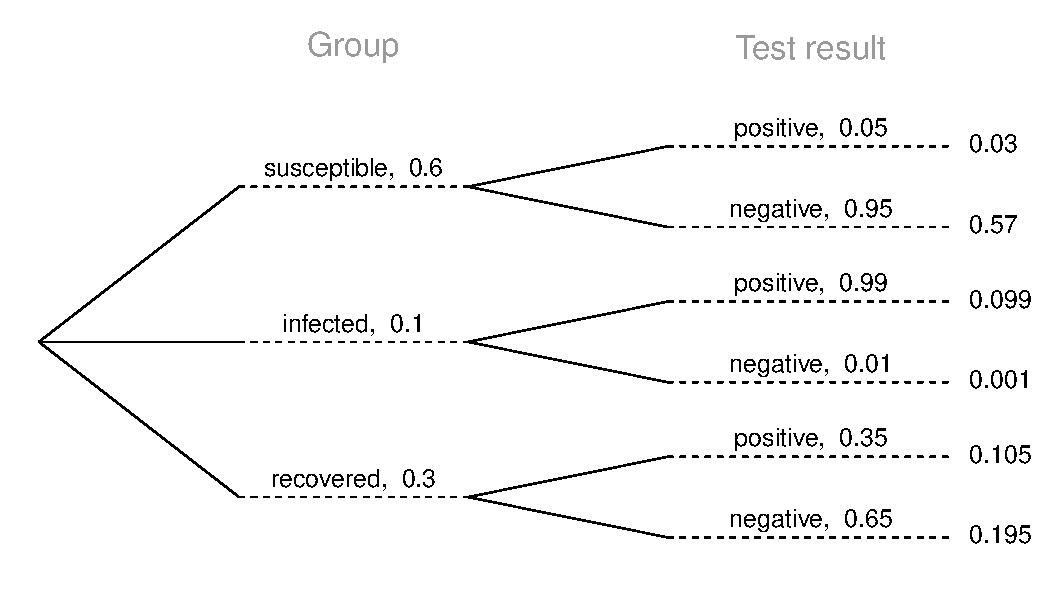
\includegraphics[width=\textwidth]{3-2_conditional_probability/figures/sir_tree/sir_tree}

\[ P(\text{感染} | +) = \frac{P(\text{感染}~\text{かつ}~+)}{P(+)} = \frac{0.099}{0.03 + 0.099 + 0.105} \approx 0.423 \]


\end{frame}

%%%%%%%%%%%%%%%%%%%%%%%%%%%%%%%%%%%%

%%%%%%%%%%%%%%%%%%%%%%%%%%%%%%%%%%%%

\section{少ない母集団からの標本抽出}

%%%%%%%%%%%%%%%%%%%%%%%%%%%%%%%%%%%%

\begin{frame}[shrink=10]
\frametitle{復元抽出}

\hl{復元抽出}では、引いたものを元に戻す。

\begin{itemize}

\item 赤チップ5個、青チップ3個、オレンジチップ2個が入った袋があるとする。最初に引いたチップが青である確率は何か？
\begin{center}
5 \textcolor{red}{$\CIRCLE$}~, 3 \textcolor{blue}{$\CIRCLE$}~, 2 \textcolor{orange}{$\CIRCLE$}
\end{center}

\[ Prob(1\text{番目のチップが青}) = \frac{3}{5 + 3 + 2} = \frac{3}{10} = 0.3 \]

\item 1回目の引きで青チップを引いたとする。復元抽出で引く場合、2回目の引きで青チップを引く確率は何か？

\begin{center}
$1\text{回目}$: 5 \textcolor{red}{$\CIRCLE$}~, 3 \textcolor{blue}{$\CIRCLE$}~, 2 \textcolor{orange}{$\CIRCLE$} \\

$2\text{回目}$: 5 \textcolor{red}{$\CIRCLE$}~, 3 \textcolor{blue}{$\CIRCLE$}~, 2 \textcolor{orange}{$\CIRCLE$}
\end{center}

\[ Prob(2\text{番目のチップが青} | 1\text{番目のチップが青}) = \frac{3}{10} = 0.3 \]

\end{itemize}

\end{frame}

%%%%%%%%%%%%%%%%%%%%%%%%%%%%%%%%%%%%%

\begin{frame}
\frametitle{復元抽出（続き）}

\begin{itemize}

\item 1回目の引きでオレンジチップを引いたとする。復元抽出で引く場合、2回目の引きで青チップを引く確率は何か？

\begin{center}
$1\text{回目}$: 5 \textcolor{red}{$\CIRCLE$}~, 3 \textcolor{blue}{$\CIRCLE$}~, 2 \textcolor{orange}{$\CIRCLE$} \\
$2\text{回目}$: 5 \textcolor{red}{$\CIRCLE$}~, 3 \textcolor{blue}{$\CIRCLE$}~, 2 \textcolor{orange}{$\CIRCLE$}
\end{center}
\[ Prob(2\text{番目のチップが青} | 1\text{番目のチップがオレンジ}) = \frac{3}{10} = 0.3 \]

\item 復元抽出で、2回続けて青チップを引く確率は何か？
\begin{center}

$1\text{回目}$: 5 \textcolor{red}{$\CIRCLE$}~, 3 \textcolor{blue}{$\CIRCLE$}~, 2 \textcolor{orange}{$\CIRCLE$} \\
$2\text{回目}$: 5 \textcolor{red}{$\CIRCLE$}~, 3 \textcolor{blue}{$\CIRCLE$}~, 2 \textcolor{orange}{$\CIRCLE$}
\end{center}
\footnotesize
\[ Prob(1\text{番目のチップが青}) \cdot Prob(2\text{番目のチップが青} | 1\text{番目のチップが青}) \]
\[ = 0.3 \times 0.3 \]
\[ = 0.3^2 = 0.09 \]

\end{itemize}

\end{frame}

%%%%%%%%%%%%%%%%%%%%%%%%%%%%%%%%%%%%%

\begin{frame}[shrink=20]
\frametitle{復元抽出（続き）}

\begin{itemize}

\item 復元抽出では、2番目のチップが青である確率は、1番目のチップの色に依存しない。なぜなら、1回目に引いたものを袋に戻すからである。
\[ Prob(\text{青} | \text{青}) = Prob(\text{青} | \text{オレンジ}) \]

\item さらに、この確率は1番目のチップが青である確率と等しい。なぜなら、復元抽出では袋の構成が変わらないからである。
\[ Prob(\text{青} | \text{青}) = Prob(\text{青}) \]

\item \hl{復元抽出では、引き操作は独立である。}

\end{itemize}

\end{frame}


%%%%%%%%%%%%%%%%%%%%%%%%%%%%%%%%%%%%%

\begin{frame}
\frametitle{非復元抽出}

\hl{非復元抽出}では、引いたものを元に戻さない。

\begin{itemize}

\item 1回目の引きで青チップを引いたとする。非復元抽出で引く場合、2回目の引きで青チップを引く確率は何か？
\begin{center}
$1\text{回目}$: 5 \textcolor{red}{$\CIRCLE$}~, 3 \textcolor{blue}{$\CIRCLE$}~, 2 \textcolor{orange}{$\CIRCLE$} \\
$2\text{回目}$: 5 \textcolor{red}{$\CIRCLE$}~, 2 \textcolor{blue}{$\CIRCLE$}~, 2 \textcolor{orange}{$\CIRCLE$}
\end{center}
\[ Prob(2\text{番目のチップが青} | 1\text{番目のチップが青}) = \frac{2}{9} = 0.22 \]

\item 非復元抽出で、2回続けて青チップを引く確率は何か？
\begin{center}

$1\text{回目}$: 5 \textcolor{red}{$\CIRCLE$}~, 3 \textcolor{blue}{$\CIRCLE$}~, 2 \textcolor{orange}{$\CIRCLE$} \\
$2\text{回目}$: 5 \textcolor{red}{$\CIRCLE$}~, 2 \textcolor{blue}{$\CIRCLE$}~, 2 \textcolor{orange}{$\CIRCLE$}
\end{center}
\footnotesize
\[ Prob(1\text{番目のチップが青}) \cdot Prob(2\text{番目のチップが青} | 1\text{番目のチップが青}) \]
\[  = 0.3 \times 0.22 \]
\[ = 0.066 \]

\end{itemize}

\end{frame}

%%%%%%%%%%%%%%%%%%%%%%%%%%%%%%%%%%%%%

\begin{frame}
\frametitle{非復元抽出（続き）}

\begin{itemize}

\item 非復元抽出では、1番目が青であった場合の2番目のチップが青である確率は、1番目のチップが青である確率と等しくない。なぜなら、袋の構成が1回目の引きの結果によって変わるからである。
\[ Prob(\text{青} | \text{青}) \ne Prob(\text{青}) \]

\item \hl{非復元抽出では、引き操作は独立でない。}

\item これは、標本サイズが小さいときに特に注意が必要である。たとえば、（巨大な）袋に10,000個のチップが入っている場合、1つのチップを引き出しても2回目の引きの確率にはそれほど大きな影響を与えない。

\end{itemize}

\end{frame}

%%%%%%%%%%%%%%%%%%%%%%%%%%%%%%%%%%%%%

\begin{frame}
\frametitle{練習問題}

\pq{ほとんどのカードゲームでは、カードは非復元で配られる。エースを引いてから3を引く確率は何か？最も近い答えを選びなさい。}

\twocol{0.3}{0.6}{
\begin{enumerate}[(a)]
\item 0.0045
\item 0.0059
\solnMult{0.0060}
\item 0.1553
\end{enumerate}
}
{
\soln{
\[ P(\text{エース次に3}) = \frac{4}{52} \times \frac{4}{51} \approx 0.0060 \]
}
}

\end{frame}

%%%%%%%%%%%%%%%%%%%%%%%%%%%%%%%%%%%%%

%%%%%%%%%%%%%%%%%%%%%%%%%%%%%%%%%%%%

\section{確率変数}

%%%%%%%%%%%%%%%%%%%%%%%%%%%%%%%%%%%%

\begin{frame}
\frametitle{確率変数}

\begin{itemize}

\item \hl{確率変数}とは、確率的事象の結果に依存する数値量のことである
\begin{itemize}
\item 確率変数を表すために $X$ のような大文字を使う
\item 確率変数の値は小文字、ここでは $x$ で表す
\item 例：$P(X = x)$
\end{itemize}

\item 確率変数には2種類ある：
\begin{itemize}
\item \hl{離散確率変数}はしばしば整数値のみをとる
\begin{itemize}
\item 例：履修単位数、今学期と前学期の履修単位数の差
\end{itemize}
\item \hl{連続確率変数}は実数（小数）値をとる
\begin{itemize}
\item 例：今学期の教科書代、今学期と前学期の教科書代の差
\end{itemize}
\end{itemize}

\end{itemize}

\end{frame}

%%%%%%%%%%%%%%%%%%%%%%%%%%%%%%%%%%%%

\subsection{期待値}

%%%%%%%%%%%%%%%%%%%%%%%%%%%%%%%%%%%%

\begin{frame}
\frametitle{期待値}

\begin{itemize}

\item 確率変数の平均的な結果にしばしば関心がある。

\item これを\hl{期待値}（平均）と呼び、可能な結果の加重平均である
\formula{\[\mu = E(X) = \sum_{i = 1}^k x_i ~ P(X = x_i)\]}

\end{itemize}

\end{frame}

%%%%%%%%%%%%%%%%%%%%%%%%%%%%%%%%%%%%

\begin{frame}
\frametitle{離散確率変数の期待値}

\dq{カードゲームで、ハートを引いたら1ドル、エース（ハートのエースを含む）を引いたら5ドル、スペードのキングを引いたら10ドル、それ以外のカードを引いたら何も得られない。勝利金の確率モデルを書き、期待される勝利金を計算しなさい。}

\begin{center}
\renewcommand{\arraystretch}{1.5}
\begin{tabular}{l | c | c | c }
事象		& $X$ 		& $P(X)$        		& $X ~ P(X)$ \\
\hline
ハート（エース以外）	& $1$		& $\frac{12}{52}$	& $\frac{12}{52}$ \\
エース			& $5$		& $\frac{4}{52}$	& $\frac{20}{52}$ \\
スペードのキング	& $10$		& $\frac{1}{52}$	& $\frac{10}{52}$ \\
その他		& $0$		& $\frac{35}{52}$	& $0$ \\
\hline
合計			&			&				& $E(X) = \frac{42}{52} \approx 0.81$
\end{tabular}

\end{center}

\end{frame}

%%%%%%%%%%%%%%%%%%%%%%%%%%%%%%%%%%%%

\begin{frame}
\frametitle{離散確率変数の期待値（続き）}

以下はこのゲームの勝利金の確率分布を視覚的に表したものである：

\begin{center}
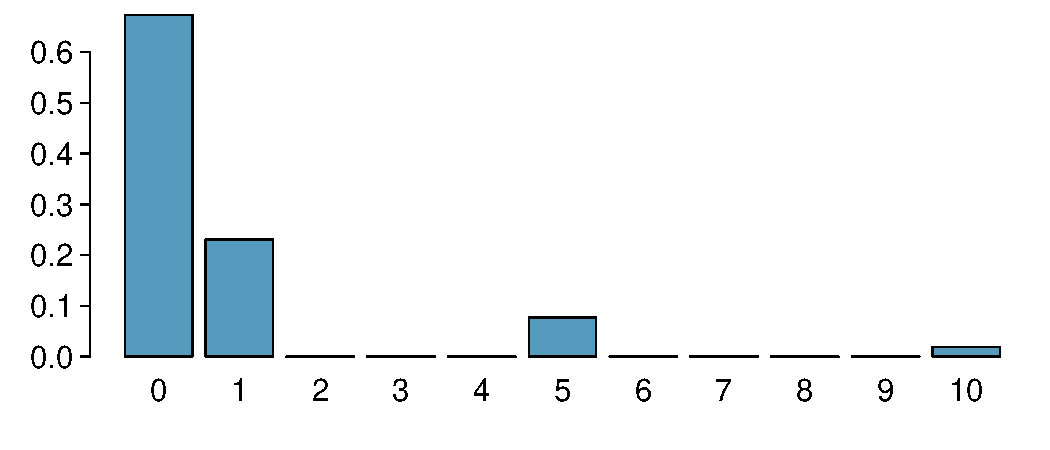
\includegraphics[width=0.8\textwidth]{3-4_random_variables/figures/card_game/card_game}
\end{center}

\end{frame}

%%%%%%%%%%%%%%%%%%%%%%%%%%%%%%%%%%%%

\subsection{確率変数の変動性}

%%%%%%%%%%%%%%%%%%%%%%%%%%%%%%%%%%%%

\begin{frame}
\frametitle{変動性}

確率変数の値の変動性にもしばしば関心がある。

\formula{
\[ \sigma^2 = Var(X) = \sum_{i = 1}^k (x_i - E(X))^2 P(X = x_i) \]
\[ \sigma = SD(X) = \sqrt{Var(X)} \]
}

\end{frame}

%%%%%%%%%%%%%%%%%%%%%%%%%%%%%%%%%%%%

\begin{frame}[shrink=15]
\frametitle{離散確率変数の変動性}

\dq{先のカードゲームの例で、ゲームごとに勝利金がどのくらい変動すると予想されるか？}

\vspace{2mm}
{\footnotesize
\begin{center}
\renewcommand{\arraystretch}{2}
\begin{tabular}{c | c | c | l | p{4cm}}
$X$ & $P(X)$         & $X ~ P(X)$      & \multicolumn{1}{c|}{$(X - E(X))^2$}  & \multicolumn{1}{c}{$P(X) ~ (X - E(X))^2$}  \\
\hline
1 & $\frac{12}{52}$  & $1 \times \frac{12}{52} = \frac{12}{52}$ & $(1 - 0.81)^2 = 0.0361$ &  $\frac{12}{52} \times 0.0361 = 0.0083$ \\
\hline
5 & $\frac{4}{52}$   & $5 \times \frac{4}{52} = \frac{20}{52}$ & $(5 - 0.81)^2 = 17.5561$  & $\frac{4}{52} \times 17.5561 = 1.3505$ \\
\hline
10  & $\frac{1}{52}$ & $10 \times \frac{1}{52} = \frac{10}{52}$  & $(10 - 0.81)^2 = 84.4561$   & $\frac{1}{52} \times 84.0889 = 1.6242$ \\
\hline
0 & $\frac{35}{52}$  & $0 \times \frac{35}{52} = 0$  & $(0 - 0.81)^2 = 0.6561$ & $\frac{35}{52} \times 0.6561 = 0.4416$ \\
\hline
  &       & $E(X) = 0.81$ & & \soln{$V(X) = 3.4246$} \\
 &       &                                                         & & \soln{$SD(X) = \sqrt{3.4246} = 1.85$} \\
\end{tabular}
\end{center}
}
\end{frame}

%%%%%%%%%%%%%%%%%%%%%%%%%%%%%%%%%%%%

\subsection{確率変数の線形結合}

%%%%%%%%%%%%%%%%%%%%%%%%%%%%%%%%%%%%

\begin{frame}
\frametitle{線形結合}

\begin{itemize}

\item 確率変数 $X$ と $Y$ の\hl{線形結合}は次のように表される

\[ aX + bY \]

ここで $a$ と $b$ はある固定された数である。

\item 確率変数の線形結合の平均値は次のように計算される
\formula{\[ E(aX + bY) = a \times E(X) + b \times E(Y) \]}

\end{itemize}

\end{frame}

%%%%%%%%%%%%%%%%%%%%%%%%%%%%%%%%%%%%

\begin{frame}
\frametitle{線形結合の期待値の計算}

\dq{統計学の宿題問題1つには平均10分、化学の宿題問題1つには平均15分かかる。今週は統計学の宿題5問と化学の宿題4問が出された。今週の統計学と化学の宿題に費やすと予想される合計時間は何か？}

\soln{
\begin{align*}
&E(S + S + S + S + S + C + C + C + C)  \\
&= 5 \times E(S) + 4 \times E(C) \\
&= 5 \times 10 + 4 \times 15 \\
&= 50 + 60 \\
&= 110~\text{分}
\end{align*}
}

\end{frame}

%%%%%%%%%%%%%%%%%%%%%%%%%%%%%%%%%%%%

\subsection{確率変数の線形結合の変動性}

%%%%%%%%%%%%%%%%%%%%%%%%%%%%%%%%%%%%

\begin{frame}
\frametitle{線形結合}

\begin{itemize}

\item 2つの独立な確率変数の線形結合の変動性は次のように計算される

\formula{\[ V(aX + bY) = a^2 \times V(X) + b^2 \times V(Y) \]}

\item 線形結合の標準偏差は分散の平方根である。

\end{itemize}

\vfill

\Note{確率変数が独立でない場合、分散の計算はやや複雑になり、本講義の範囲を超える。}

\end{frame}

%%%%%%%%%%%%%%%%%%%%%%%%%%%%%%%%%%%%

\begin{frame}
\frametitle{線形結合の分散の計算}

\dq{統計学の宿題問題1つにかかる時間の標準偏差は1.5分、化学の宿題問題1つには2分である。統計学の宿題5問と化学の宿題4問が出された今週に統計学と物理学の宿題に費やすと予想される時間の標準偏差は何か？各問題にかかる時間は互いに独立であると仮定する。}

\soln{
\begin{align*}
&V(S + S + S + S + S + C + C + C + C)  \\
&= V(S) + V(S) + V(S) + V(S) + V(S)  \\
&+ V(C) + V(C) + V(C) + V(C) \\
&= 5 \times V(S) + 4 \times V(C) \\
&= 5 \times 1.5^2 + 4 \times 2^2 \\
&= 27.25
\end{align*}
}

\end{frame}

%%%%%%%%%%%%%%%%%%%%%%%%%%%%%%%%%%%%

\subsection{まとめ}

%%%%%%%%%%%%%%%%%%%%%%%%%%%%%%%%%%%%

\begin{frame}[shrink=20]
\frametitle{練習問題}

\pq{カジノゲームのプレイに5ドルかかる。最初に引いたカードが赤であれば、2枚目のカードを（非復元で）引ける。2枚目がクラブのエースであれば500ドルを獲得する。そうでなければ、何も得られず（5ドルを失う）。このゲームをプレイしたときの期待利益/損失は何か？ {\small 覚えておこう：利益/損失 = 賞金 - コスト。}}

\begin{multicols}{2}
\begin{enumerate}[(a)]
\item 5セントの利益
\solnMult{10セントの損失}
\item 25セントの損失
\item 30セントの損失
\end{enumerate}
\end{multicols}

\soln{
{\small
\renewcommand\arraystretch{1.25}
\begin{tabular}{l c c c r}
事象				& 賞金	& 利益: $X$	& $P(X)$	& $ X \times P(X)$	\\
\hline
\orange{赤}, {A}{$\clubsuit$}		& 500		& 500 - 5 = 495	& $\frac{26}{52} \times \frac{1}{51} = 	0.0098$ & 	 $495 \times 0.0098 = 4.851$ \\
その他	& 0 			& 0 - 5 = -5	& $1 - 0.0098 = 0.9902$ & $-5 \times 0.9902 = -4.951$ \\
\hline
					&			&			& 			& $E(X) = -0.1$
\end{tabular}
}
}

\end{frame}

%%%%%%%%%%%%%%%%%%%%%%%%%%%%%%%%%%%%

\begin{frame}[shrink=10]
\frametitle{公正なゲーム}

\hl{公正な}ゲームとは、コストが期待される賞金額と同じ、すなわち期待利益が0のゲームである。

$\:$

\dq{ラスベガスのカジノゲームは、期待される賞金額より多くかかると思うか、少なくかかると思うか？}

\soln{
\begin{columns}[c]
\column{0.6\textwidth}
もしそれらのゲームが期待される賞金額より少なければ、カジノは平均的に損をしていることになり、以下のようなものに費用を払えなくなる：
\column{0.4\textwidth}
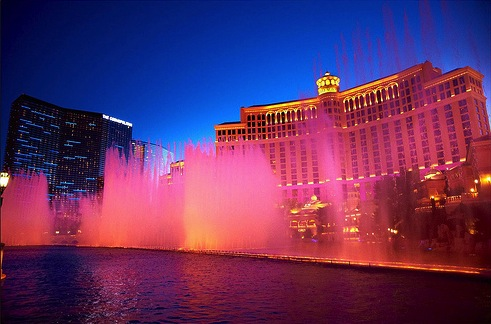
\includegraphics[width=\textwidth]{3-4_random_variables/figures/bellagio.jpg}
\end{columns}
\ct{Image by Moyan\_Brenn on Flickr \webURL{http://www.flickr.com/photos/aigle\_dore/5951714693}.}
}


\end{frame}

%%%%%%%%%%%%%%%%%%%%%%%%%%%%%%%%%%%%%

\begin{frame}
\frametitle{確率変数の簡略化}

確率変数は通常の代数変数とは異なる振る舞いをする：
\[ X + X \ne 2X \]

{\small
\twocol{0.45}{0.45}
{
\begin{align*}
E(X + X) &= E(X) + E(X) \\
&= 2 E(X) \\
&~  \\
E(2X) &= 2 E(X) \\
&~
\end{align*}
}
{
\begin{align*}
Var(X + X) &= Var(X) + Var(X)~{\scriptsize \text{（独立を仮定）}} \\
&= 2~Var(X) \\
&~  \\
Var(2X) &= 2^2~Var(X) \\
&= 4~Var(X)
\end{align*}
}
}

\vspace{3mm}

\mathhl{E(X + X)  = E(2X)} だが、\mathhl{Var(X + X) \ne Var(2X)} である。

\end{frame}

%%%%%%%%%%%%%%%%%%%%%%%%%%%%%%%%%%%%%

\begin{frame}[shrink=25]
\frametitle{足し算か掛け算か？}

\dq{ある会社のフリートに5台のリンカーン・タウンカーがある。過去のデータによると、各車の年間メンテナンスコストは平均2,154ドル、標準偏差は132ドルである。このフリートの年間総メンテナンスコストの平均と標準偏差は何か？}

1台の車が年間メンテナンスコストの5倍 $(5X)$ ではなく、それぞれ同じ年間メンテナンスコストを持つ5台の車 $(X_1 + X_2 + X_3 + X_4 + X_5)$ であることに注意する。

{\small
\begin{eqnarray*}
E(X_1 + X_2 + X_3 + X_4 + X_5) &=& E(X_1) + E(X_2) + E(X_3) + E(X_4) + E(X_5) \\
&=& 5 \times E(X) = 5 \times 2,154 = \$ 10,770 \\
Var(X_1 + X_2 + X_3 + X_4 + X_5) &=& Var(X_1) + Var(X_2) + Var(X_3) + Var(X_4) + Var(X_5) \\
&=& 5 \times V(X) = 5 \times 132^2 = \$ 87,120 \\
SD(X_1 + X_2 + X_3 + X_4 + X_5) &=& \sqrt{87,120} =  295.16
\end{eqnarray*}
}

\end{frame}

%%%%%%%%%%%%%%%%%%%%%%%%%%%%%%%%%%%%

%%%%%%%%%%%%%%%%%%%%%%%%%%%%%%%%%%%%

\section{連続分布}

%%%%%%%%%%%%%%%%%%%%%%%%%%%%%%%%%%%%

\begin{frame}[shrink=15]
\frametitle{連続分布}

\begin{itemize}

\item 以下は米国成人の身長の分布のヒストグラムである。

\item 陰影のついたビンに含まれるデータの割合が、無作為に選ばれた米国成人の身長が180cmから185cm（約5'11''から6'1''）である確率を示す。

\end{itemize}

\begin{center}
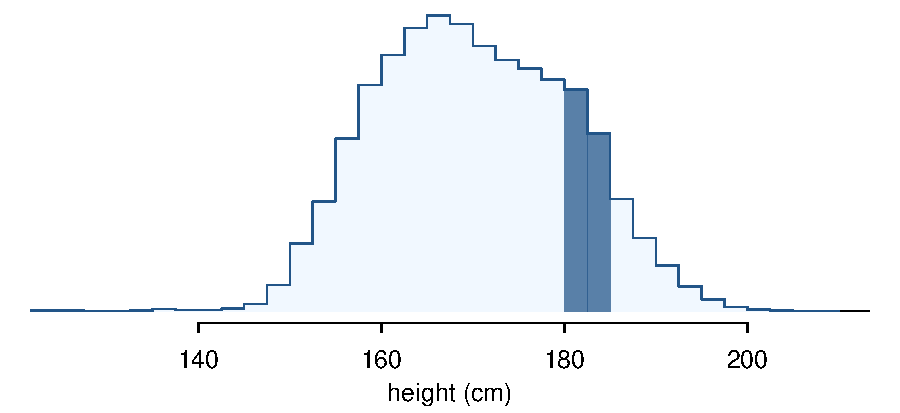
\includegraphics[width=\textwidth]{3-5_continuous_distributions/figures/usHeightsHist180185/usHeightsHist180185}
\end{center}


\end{frame}

%%%%%%%%%%%%%%%%%%%%%%%%%%%%%%%%%%%%

\subsection{ヒストグラムから連続分布へ}

\begin{frame}
\frametitle{ヒストグラムから連続分布へ}

身長は連続数値変数であるため、その\hl{確率密度関数}は滑らかな曲線となる。

\begin{center}
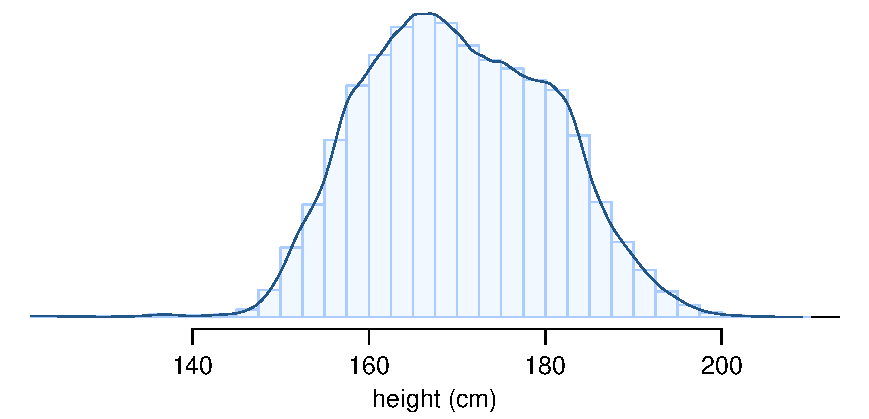
\includegraphics[width=\textwidth]{3-5_continuous_distributions/figures/fdicHeightContDist/fdicHeightContDist}
\end{center}

\end{frame}

%%%%%%%%%%%%%%%%%%%%%%%%%%%%%%%%%%%%

\subsection{連続分布からの確率}

\begin{frame}[shrink=10]
\frametitle{連続分布からの確率}

したがって、無作為に選ばれた米国成人の身長が180cmから185cmである確率は、曲線の下の陰影部分の面積としても推定できる。

\begin{center}
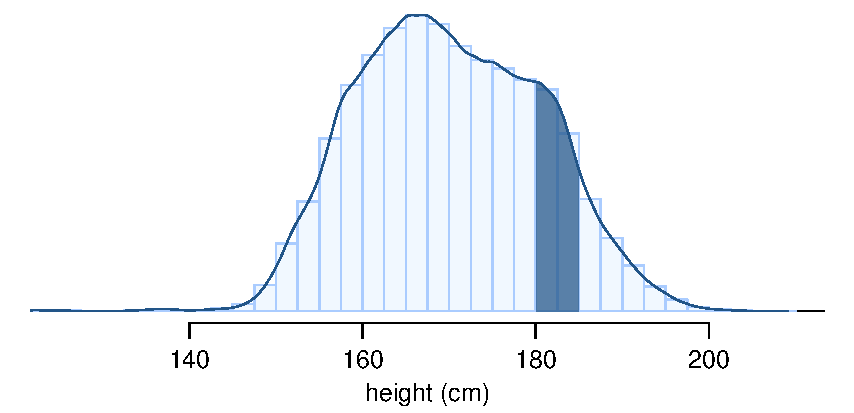
\includegraphics[width=\textwidth]{3-5_continuous_distributions/figures/fdicHeightContDistFilled/fdicHeightContDistFilled}
\end{center}


\end{frame}

%%%%%%%%%%%%%%%%%%%%%%%%%%%%%%%%%%%%

\begin{frame}
\frametitle{定義によれば…}

連続確率は「曲線の下の面積」として推定されるため、ある人の身長がちょうど180cm（または任意の特定の値）である確率は0と定義される。

\begin{center}
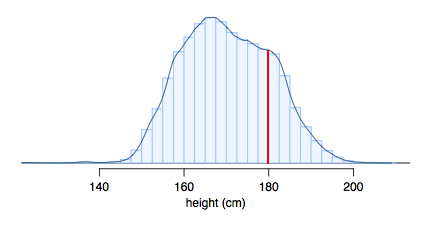
\includegraphics[width=0.8\textwidth]{3-5_continuous_distributions/figures/fdicHeightContDist180}
\end{center}

\end{frame}

%%%%%%%%%%%%%%%%%%%%%%%%%%%%%%%%%%%%



%%%%%%%%%%%%%%%%%%%%%%%%%%%%%%%%%%%%
% ドキュメント終了
%%%%%%%%%%%%%%%%%%%%%%%%%%%%%%%%%%%%

\end{document}
